\section{Full simulasjon}
\thispagestyle{fancy}
\begin{figure}[htbp]
    \centering
    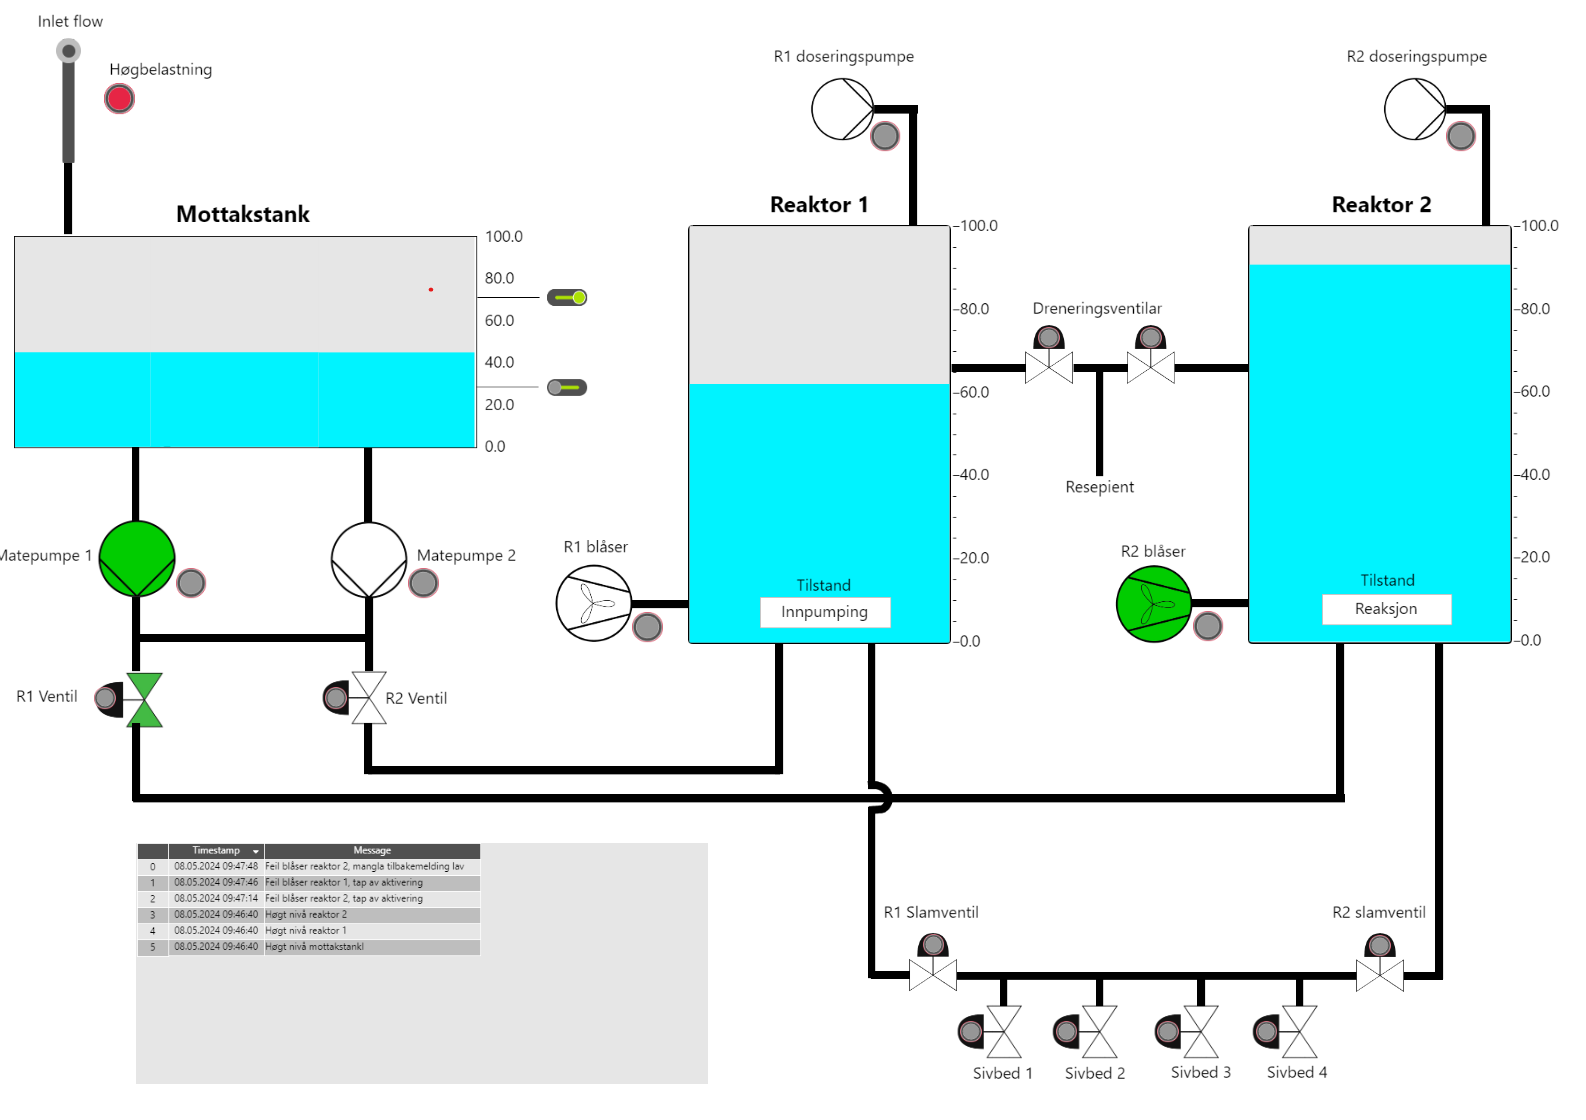
\includegraphics[width=1\textwidth]{Bilder/Simuleringsbilde.png}
    \caption{Oppsett av simuleringsvindu}\label{fig:Simulering}
\end{figure}
\subsection{Oppsett}
Med simulasjonsblokkene klare og eit simuleringsvindu og vise resultat på var vi
no klare for å sette opp ein fullstending simulasjon av anlegget.
Vi satte inn ventil tilbakemeldingsblokka på alle ventilar i programmet og oppretta eit
nytt CFC vindu som kopla tank simuleringa av mottakstanken og reaktorane ilag med resten av
programmet.

Simulasjonen er satt opp slik at tilstrøymning til anlegget kan stillast av ein glidar.
Dersom ein av reaktorane er i innpumpings sekvens simulerast vi flytting av avlaupsvatn
basert på pumpekurver og løftehøgder.

Reaktortilstand er representert ved ein teksvariabel og
dei aktuelle tidsparameterane, som eksempelvis tid på reaksjonssekvens,
er redusert for å akselerere simuleringen.

Vi har også lagt til ein alarmlogg for alle moglege alarmar anlegget kan generere, 
uavhengig om dei er aktuelle å ha med i sluttprogrammet eller ikkje.
Dette gjer oss verdifull innsikt i korleis programmet fungera.



\subsection{Resultat}


Før simuleringa starta vart programmet satt opp for å bli simulert. 
Dette betyr at vi i første simuleringsfase, ikkje simulerer ein fullskala test, men at vi skalerer ned volumet i tankane 
for å få ned tida det tar å simulere ein full syklus av begge reaktorane. 
Som forventa dukk det opp nokre avvik når vi begynte å simulere. 
Nokre av desse var av mindre betydning og utbetra  undervegs, som for eksempel at våra forrigling av reaktortankane ikkje skal 
kunne gå i innpumpingstilstand samstundes, ikkje fungerte.

Våra fullskala simulering var veldig vellykka. 
Vi fekk samla masse verdifull data av anlegget i simulert drift, og vi fekk verifisert våra kode fungerte som planlagt. 
Den visuelle representasjonen var oversiktleg og ein kunne lett sjå koden i drift og visuelt forstå kva koden våra gjorde.      


Her bør det stå litt av resultata av simulering? \newline
Kanskje eksempel på litt kva vi såg osv.\newline
